\chapter{Metod}
I det här avsnittet beskriver vi metodiken för utvecklandet av webbsidan, utvecklandet av djupinlärningsalgoritmerna samt experimentet för att undersöka interaktionen mellan studenter och artificiell intelligens. Speciellt betonas iterationsprocessen mellan produktutveckling och webbutveckling samt datamängden som utgör en grund till utvecklingen av djupinlärningsalgoritmerna.

\section{Produkt- och webbutveckling}

I följande avsnitt presenteras först de förutsättningar som gör att metoden ser ut på det sätt den gör. Därefter redogörs metoden för produkt- och webbutvecklingen.  

Projektets utformning skapar utmaningen att på snabbast möjliga tid skapa en fullt fungerande och skalbar hemsida. Hemsidan måste vara fullt fungerande av två skäl. För det första, eftersom den måste användas i en riktig situation för att få verkliga data på studenternas studiemönster för att kunna ge korrekta förutsägelser. För det andra, för att undvika att utveckla funktionalitet som inte fungerar i en verklig användningssituation. Hemsidan måste också vara skalbar, dvs det ska gå att öka antalet kurser och användare på sidan utan att skapa problem. Tidskravet är viktigt eftersom projektet förhåller sig till de naturliga deadlines som de faktiska kurserna sätter, såsom kursstart och tentavecka. 

För att fullt optimera arbetsflödet mellan produkt- och webbutvecklingen krävdes ett strukturerat informationsflöde, samt tydliga processer. I ett tidigt skede bestämde de båda spåren att ha möten där idéer, målsättningar och krav formellt diskuterades. Utöver dessa möten användes Figma för att visualisera prototyper designmässigt. Webbutvecklingsgruppen använde därefter filer från Figma för att designa applikationen. En anslagstavla skapades i Trello, där produktutvecklaren kunde distribuera arbetsmoment som webbutvecklingsgruppen skulle iterera över. Parallellt med ovan nämnda informationskanaler användes Slack för att i realtid diskutera pågående problem, beslut och uppdateringar.

Utifrån det ovan nämnda tidskravet, gjordes det på förhand intervjuer med föreläsare samt en utvärdering av elevers användande av programmen MapleTA och OpenTA. Även gjordes en så kallad benchmarking av andra internetbaserade inlärningsprogram för att få en uppfattning om rådande design och funktionalitet. Utifrån denna information gjordes en design av hemsidans gränssnitt som grund för att utveckla en fullt fungerande prototyp.

En minimalt funktionell hemsida utvecklades utifrån kraven samt designriktlinjerna. Denna hemsida testades sedan i slutet av läsperiod 3 i en kurs genom att lägga in gamla tentor på hemsidan och frivilligt låta studenterna använda den. Efter detta utvärderades hemsidan med de studenter som använt hemsidan i form av intervjuer. Feedbacken från intervjuerna återkopplades till utvecklingen. 

Parallellt med utvecklingen av grundfunktionaliteten gjordes ytterligare en informationsinsamling i form av semistrukturerade intervjuer kring plattformen Piazza. Dessa intervjuer transkriberades varefter en workshop hölls där nyckelcitat extraherades och en KJ-analys gjordes på citaten, se diagram x. Utifrån detta och den tidigare insamlade informationen togs ett par koncept fram på eventuella lösningar. Varav en av dessa bestämdes för att gå vidare med, härefter kallad MVP A. 

%Stycke om metod-utveckling av MVP-A
Efter utvärderingsprocessen användes resultaten för att skapa en utökning på dåvarande MVP. I ett tidigt skede skulle en större omstrukturering av kod vara nödvändig, eftersom många designbeslut baserats på att få igång systemet på kortast möjliga tid. Att prioritera enkelhet bidrar i flesta fall till att ett system inte skalar optimal. Efter rensningen påbörjades det experimentella arbetet att skapa funktionalitet som både kunde bidra till att förbättra studieresultat, men även användas i deep learning-algoritmen för att ge en bättre säkerhet. Utvecklingsprocessen utfördes, som ovan nämnt, iterativt tillsammans med produktutvecklingen. 

Hemsidan testades sedan i två kurser från start i läsperiod 4 där kursens rekommenderade uppgifter lades in på sidan. Studenterna informerades att om de använde sidan skulle de få möjlighet att få en förutsägelse på sitt tentaresultat, halvvägs igenom läsperioden. Läsvecka 3 var MVP A färdigutvecklad och denna introducerades då till studenterna. 

%(AI metod mm)


%(Slut AI metod)
Halvvägs igenom läsperioden gavs studenterna deras förutspådda tentaresultat genom att ta in dem i enrum och visa dem resultatet följt av en intervju. På grund av att det var stor osäkerhet i hur faktiska testerna skulle utspela sig, gjordes också intervjuer allmänt kring studenternas inställning till att få sina studieresultat förutspådda. Detta genom semistrukturerande intervjuer. 


% \section{Metod Deep Learning}

% OpenTA-datan bearbetades med hjälp av Numpy till en tredimensionell tensor på formen (\textit{antal användare}, \textit{uppgifter}, \textit{egenskaper}). För varje användare finns alltså en matris bestående av alla uppgifter och för varje uppgift finns ett antal egenskaper. Dessa egenskaper extraherades ur datan med hjälp av script i Python samt databehandlingspaketet Pandas (se Appendix hum-hum för kod). För att identifiera ifall en egenskap var korrelerad med en elevs kursprestation användes statistisk analys... (beskrivning av analys här) ...De egenskaper som valdes ut för varje uppgift var:

% \begin{itemize}
%     \item Rätt eller fel
%     \item Antal försök 
%     \item Tidpunkt i kursen då uppgiften påbörjades 
%     \item Medeltid mellan försök 
%     \item Total tid spenderad
% \end{itemize}

% Därefter tränades neurala nätverk mot denna data. De två nätverkstyper som studerades var djupa neurala nätverk, DNN, samt Long-Short-Time-Memory-nätverk, LSTM. Olika kombinationer av dessa två nätverkstyper testades, och jämfördes mot varandra samt en grundnivå. Som grundnivå valdes andelen underkända i kursen, 60\%, då det motsvarar träffsäkerheten om man bara hade gissat att alla i kursen var godkända. För att utvärdera nätverkens prestanda på den lilla datamängden delades användarna slumpmässigt in i tränings- och valideringsdata. Nätverket tränades på träningsdatan och evaluerades på evalueringsdatan, varpå högsta valideringsträffsäkerheten noterades. Därefter slumpades alla användare på nytt och processen upprepades. Genmom att upprepa detta 25 gånger och sedan beräkna medelvärde och standardavvikelse kunde ett relativt tillförlitligt mått på nätverkens prestanda erhållas. 

% Vidare analys utfördes även på enstaka nätverk för att med konventionella statistiska metoder finna vilka användare nätverket klassificerar felaktigt, och ifall det finns någon gemensam nämnare för dessa. 

% \begin{itemize}
%     \item Huvudmål: Beskriva datan och förklara dataflödet
%    \item Ingående data 
%    \item Processandet av data 
%    \item Analys av data 
%     \item Genera tensor
%\end{itemize}

\section{Metodbeskrivning: Utveckling av djupinlärningsalgoritmer}

\subsection{Databeskrivning och databehandling}
Vår data har två källor, OpenTA och vår egenutveckalde applikation YATA. Därav behövde vi utveckla ett dataflöde som kan processa data från båda källorna och samtidigt kunna skala i enhet med vår egen applikation. Eftersom vi hade tillgång till OpenTA-datan först valde vi att låta den diktera huvudformatet på dataflödet. Därav beskriver föjande text dataflödet och databehandlingen för båda källorna. OpenTA-datan är utdrag från OpenTA:s server och innehåller data från studenter i två kurser, FFM521 år 2017 samt FFM234 år 2018. Datan representerar 152 respektive 101 studenter. En datarad består av 4 attribut; användare, uppgift, om studentens försök var korrekt och tid vid försök. Dessa attribut processade vi om till 5 egenskaper (eng. \textit{features}) för att resultera i en tensor som kan användas till att träna våra neurala nätverk. Exakta formen på tensorn bestämdes till (\textit{unika användare}, \textit{unika uppgifter}, \textit{egenskaper}). För varje användare finns en matris med rader som  motsvarar unika uppgifter och kolumner som motsvarar våra fem egenskaper. 
Dessa egenskaper extraherades med hjälp av kod skriven i Python. Koden bröts ned i flera del moment enligt figur \ref{fig:dataflow}. Huvudsakligen användes databehandlingspaketet Pandas och Numpy för att behandla datan. Detta gav oss mer kontroll över dataflödet och möjligheter att integrera och skala med YATA. Detta gjorde också att vi kunde spara datan vid flera steg i processen vilket öppnar upp för mer avancerad dataanalys.

\begin{figure}[H]
    \centering
    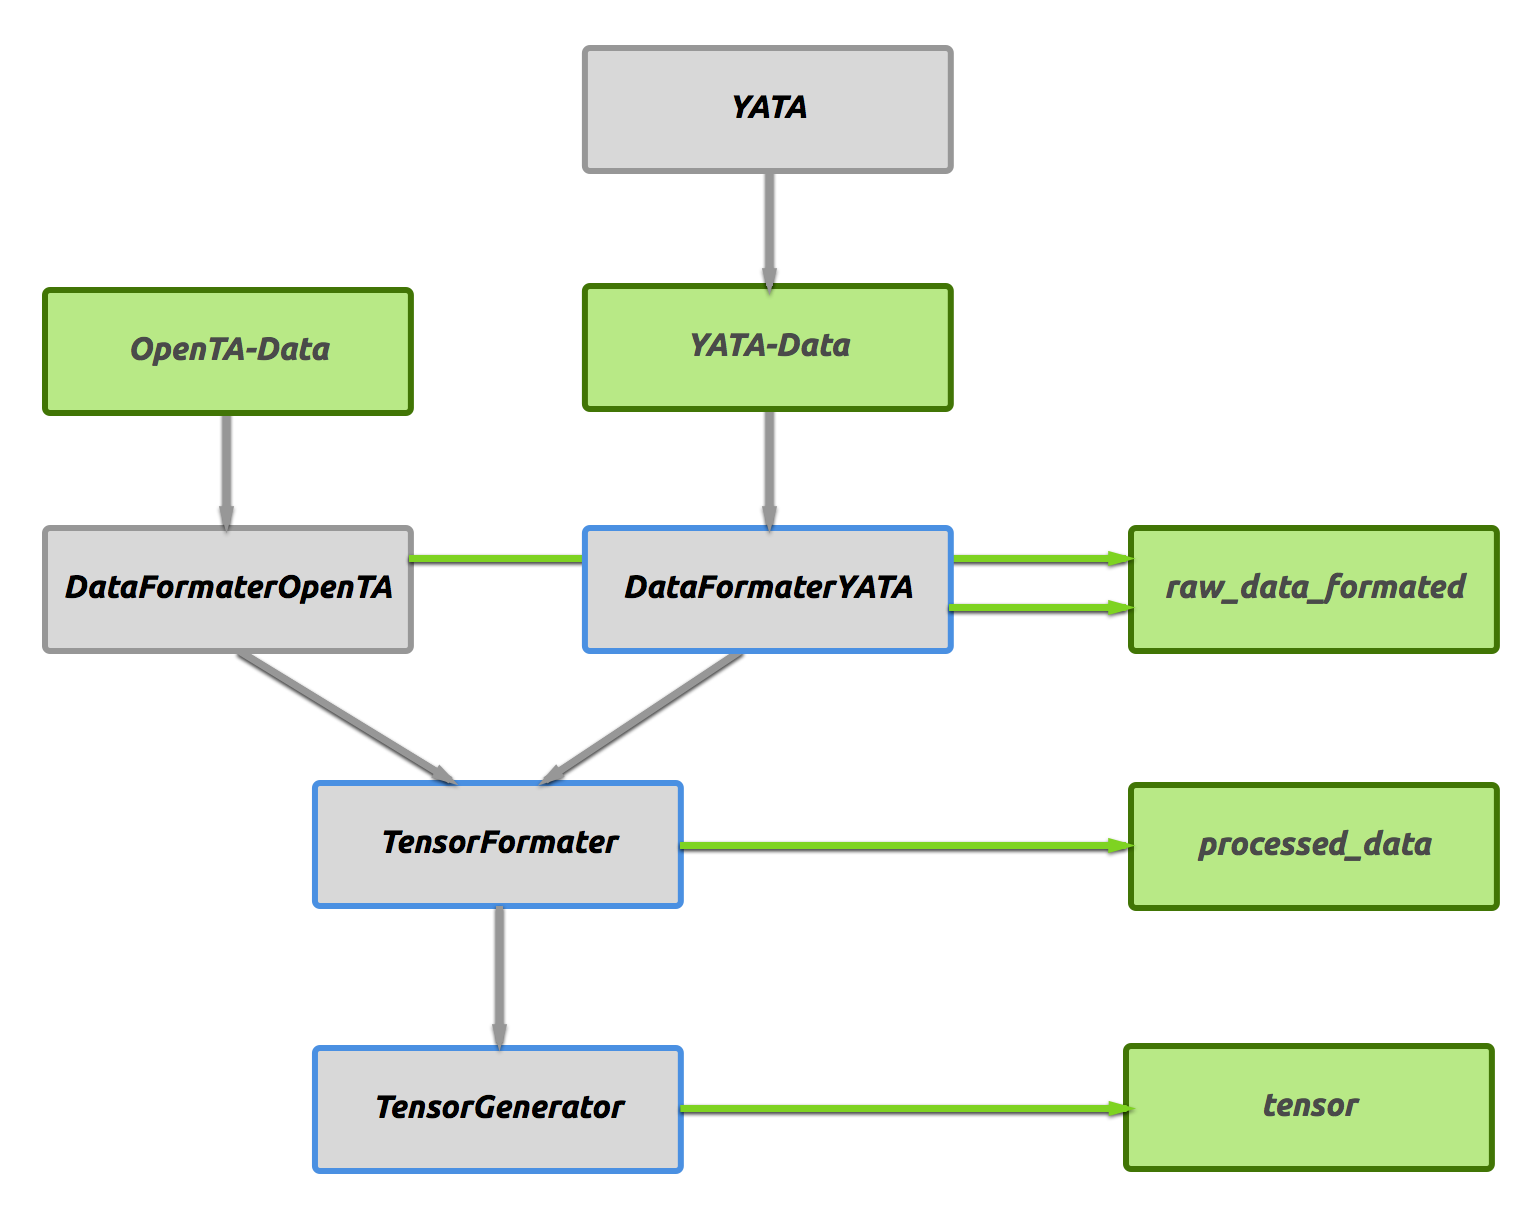
\includegraphics[width=0.5\textwidth]{images/methodpictures/dataflow.png}
    \caption{''Dataflödet'' (OBS: PALCEHOLDER, EJ FINAL).}
    \label{fig:dataflow}
\end{figure}


% Varför pandas?
% Skalar
% Hastighet
% Utvecklings potential
% Inbyggda plotfunktioner

% Varför flera filer och intern filstrktur?
% För att det möjlig gör analys av datan vid alla skeden av processen. 

% Nämna filstruktur? 
% DataFormaterOpenTA
% DataFormaterYATA
% TensorFormater
% TensorGenerator


Detta gjordes för varje kurs och för två olika tidsintervall. Ett tidsintervall motsvarade en hel läsperiod, från startdatum till tentamensdatum, och ett annat för en halv läsperiod, från startdatum till datum och tid då halva kursen hade gått. 

De extraherade värdena för respektive egenskap i datatensorn normaliserades sedan över alla användare till en $N(0,1)$-fördelningen. Motsvarande måldata erhölls genom normering av resultatdatan för alla användare. Resultatdatan normerades olika beroende på vilket problem som skulle lösas. För G/U-problemet var måldatan binär 0 eller 1, där 0 motsvarade underkänt och 1 godkänt. För U-5 utfördes en så kallad one-hot-kodning (eng. \emph{one-hot encoding}). En lista med längd fyra definierades för varje användare, med värde 0 på alla platser utom den som motsvarade det betyg eleven fick där värdet var 1.

%De extraherade värdena för respektive egenskap i datatensorn normaliserades sedan över alla användare till en $N(0,1)$-fördelningen. Användarna delades in in två delar; träningsdata och valideringsdata. För att undvika kontaminering av valideringsdatan beräknades medelvärde och standardavvikelse för respektive egenskap endast över träningsdatan, varefter all data transformerades till $N(0,1)$ genom beräkningen $N\left(\frac{\mathbb{X}-\mu}{\sigma}\right)$. 
 
\subsection{Dataanalys}

För att få fram vilka egenskaper som kunde vara relevanta att använda i våra neurala nätverk användes korrelationskoefficienter för varje enskild egenskap samt multikorrelationer för alla egenskaper. Utöver detta användes även punktdiagram tillsammans med regressionslinjer för att få fram korrelationer visuellt. Tentamensresultat gjordes om till att endast visa ifall en elev blev godkänd eller underkänd alternativt till att endast visa vilket betyg eleven fick. Detta eftersom vi ville börja med att analysera enkla neurala nätverk och se hur pass väl dessa förutsäger godkänt eller underkänt alternativt betyg för en elev. Därefter plottade vi för varje elev deras tentamensresultat mot egenskaper som vi misstänkte kunde vara intressanta. Detta, tillsammans med korrelationskoefficienter, gav oss ett verktyg för att bestämma vad som kan vara bra att träna nätverken med. Vi bestämde oss för att en korrelation på mindre än 0.25 indikerar en svag korrelation och att vi därför skulle välja bort egenskaper som gav en korrelation på mindre än 0.25. Vår hypotes var att en egenskap som har en svag korrelation ger inte upphov till stora förbättringar i nätverkens förmåga att förutsäga tentamensresultat. Dessa egenskaper medför snarare en onödig storleksökning av tensorn och därigenom en ökad beräkningskraft för en dator. De egenskaper som valdes ut för varje uppgift var:

\begin{itemize}
    \item Rätt eller fel
    \item Antal försök 
    \item Tidpunkt i kursen då uppgiften påbörjades 
    \item Medeltid mellan försök 
    \item Total tid spenderad
\end{itemize}

Alla dessa fem egenskaper klarade av vår korrelationsgräns och användes därför i alla våra nätverk. 

För att ytterligare analysera trender i datan valde vi att använda oss av stapeldiagram och plotta global data som exempelvis totalt antal rätt eller totalt antal försök. Detta plottades för varje användare och vi använde oss av en färgkodning för att indikera hur eleven presterade i kursen.

Korrelationerna vi använde oss av kollar endast på linjära samband mellan variabler. Nätverken kollar på alla möjliga samband, linjära som icke-linjära. Därav borde nätverken kunna ge bättre förutsägelser än vad korrelationerna ger. En annan rimlig hypotes är att ju högre R-värde vi har, det vill säga ju högre multikorrelation vi har, desto bättre förutsägelser borde vi få. 

Efter att datatensorer och nätverksarkitekturer var färdigställda utfördes även en felanalys över vilka användare som nätverken felaktigt klassificeradeför G/U- och U5-problemet. En felaktigt klassificerad användare är en användare som får annat betyg än vad nätverket uppskattat. Användarna i datatensorn blandades och delades därefter in i tränings- samt valideringsdata. Nätverket för det aktuella problemet tränades på träningsdatan varefter en förutsägelse på all valideringsdata gjordes. Genom att jämföra med användarna i valideringsdatans verkliga resultat kunde felaktigt klassificerade användare identifieras. För varje sådan användare extraherades totala antalet räknade uppgifter, totala antalet försök, total spenderad tid samt vilket betyg nätverket förutsagt. Detta upprepades sedan för totalt tio olika blandningar av användarna. Den extraherade datan medelvärdesbildades sedan över dessa blandningar, varefter slutsatser kring hur nätverken klassificerar användare kunde dras. 

\subsection{Träning och validering}

De neurala nätverk som har använts designades med hjälp av applikationsprogrammeringsgränssnittet Keras. Keras är ett högnivågränssnitt som implementerar Tensorflow, ett öppet maskininlärningsbibliotek från Google, och förenklar mycket av den syntax som är associerad med TensorFlow. Totalt designades tre neurala nätverk, ett för vardera av de tre problemen som vi valt att angripa. 

Nätverken tränades på ca 2/3 av OpenTA-datan för kursen FFM521 och validerades på den återstående tredjedelen. Utgångsmodellen bestod exempelvis endast av ett tätt lager, varefter lagerstorleken ökades samt fler lager lades till tills en tydlig överanpassning mot träningsdatan kunde observeras. Med hjälp av en kombination av avhopp, viktregularisering samt finjustering av hyperparametrar kunde ett optimerat nätverk erhållas.

För att validera nätverkens prestanda implementerades en egendesignad variant av k-faldig korsvalidering, då den låga datamängden ledde till att nätverkens prestanda på valideringsdatan var starkt beroende av vilka användare som utgjorde träningsdata och valideringsdata. Både datatensorn och måldatatensorn blandades varefter de delades in i tränings- och valideringsdata. Därefter tränades nätverket på träningsdatan och evaluerades mot valideringsdatan, varpå maximala och minimala värden på valideringsträffsäkerhet samt valideringsförlust sparades. Detta upprepades för 25 unika slumpningar av ordningen på data- och måldatatensorerna, varefter medelvärde och standardavvikelse för maximala och minimala värden av valideringsträffsäkerhet och valideringsförlust kunde beräknas. Dessa kunde sedan användas som kvantitativa mått på nätverkets prestanda, vilka uppvisade mindre varians än nätverkets prestanda för enstaka blandningar av data- och måldatatensorn.

\subsubsection{Nätverksarkitektur för U/G}
\label{sec:gu}
\begin{figure}[H]
    \centering
    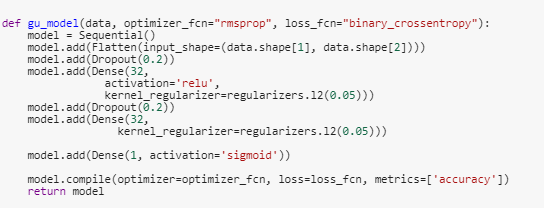
\includegraphics[width=0.7\textwidth]{images/methodpictures/gu_placeholder.png}
    \caption{Nätverksarkiktetkuren för G/U (PLACEHOLDER).}
    \label{fig:gu_model}
\end{figure}
För G/U-problemet valdes nätverksarkitekturen som ges i figur \ref{fig:gu_model}. Indatan på matrisform omvandlades först till radvektorer med hjälp av tillplattningslagret, varefter den behandlades av två dolda täta lager med 32 noder vardera med aktiveringsfunktion \emph{ReLU}. Dessa dolda täta lager var även viktregulariserade, vilket i kombination med avhopps-lagren innan dem motverkade överanpassning. Sista lagret var ett dolt tätt lager med en nod samt \emph{sigmoid}-aktivering, vilket gav att utvärdet från det neurala nätverket blev ett tal mellan 0 och 1. Detta tal motsvarar nätverkets uppskattade sannolikhet att en given student får godkänt i kursen. \emph{Binary crossentropy} valdes som förlustfunktion och \emph{RMSProp} valdes som optimeringsalgoritm. 


\subsubsection{Nätverksarkitektur för U/3/4/5}
\label{sec:u5}
\begin{figure}[H]
    \centering
    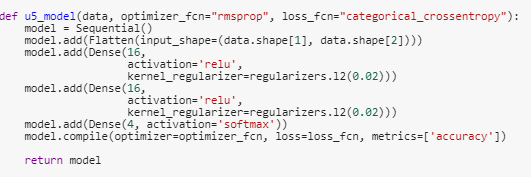
\includegraphics[width=0.7\textwidth]{images/methodpictures/u5_placeholder.png}
    \caption{Nätverksarkiktetkuren för U-5 (PLACEHOLDER).}
    \label{fig:u5_model}
\end{figure}

Nätverksarkitekturen för U5-problemet ges i figur \ref{fig:u5_model}. Nätverket består av ett tillplatningslager samt två dolda täta lager med 16 noder vardera och \emph{ReLU}-aktivering. För att motverka överanpassning var dessa lager även viktregulariserade. Det sista lagret bestod av ett dolt tätt lager med fyra noder med \emph{softmax}-aktivering. Vardera av dessa noder kan därmed anta ett värde mellan 0 och 1 (med total summa 1 över alla fyra), vilket svarar mot nätverkets uppskattning för att en given student får ett av de fyra betygen U-5. \emph{Categorical crossentropy} valdes som förlustfunktion och \emph{RMSProp} valdes som optimeringsalgoritm. 



\subsubsection{Nätverksarkitektur för skrivningspoäng och osäkerhetsnätverk}
\label{sec:exam_score}
\begin{figure}[h]
    \centering
    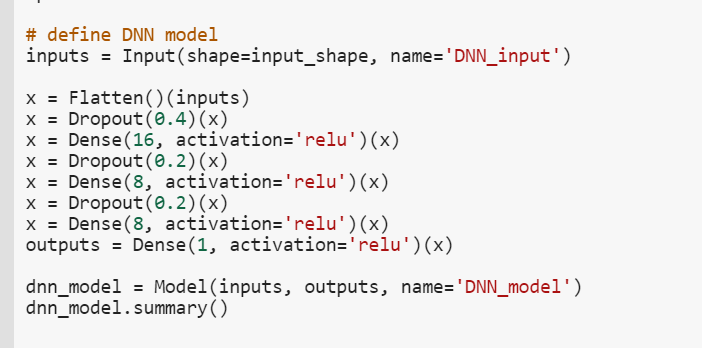
\includegraphics[width=0.7\textwidth]{images/methodpictures/poang-ffm234.PNG}
    \caption{Nätverksstrukturen för skrivningspoäng i FFM234. (PLACEHOLDER)}
    \label{fig:exam_score_ffm234}
\end{figure}

I figur \ref{fig:exam_score_ffm234} presenteras nätverksstrukturen för att förutsäga skrivningspoäng för kursen FFM234. Nätverket bestod av tre dolda täta lager med 16, åtta respektive åtta noder med aktiveringsfunktion \emph{ReLU}. För att motverka överanpassning användes avhopp för indatan till varje dolt tätt lager. Förlustfunktionen valdes till \emph{MSE} och optimeringsalgoritmen valdes till \emph{RMSprop}.

\begin{figure}[h]
    \centering
    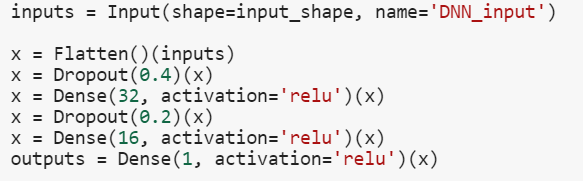
\includegraphics[width=0.7\textwidth]{images/methodpictures/poang-ffm521.PNG}
    \caption{Nätverksstrukturen för skrivningspoäng i FFM521. (PLACEHOLDER)}
    \label{fig:exam_score_ffm521}
\end{figure}
Analogt med nätverksarkitekturen för kursen FFM234 valdes förlustfunktionen \emph{MSE} och optimeringsalgoritmen \emph{RMSprop}. Däremot utgjordes nätverket av två dolda täta lager med 32 respektive 16 noder, vilket presenteras i figur \ref{fig:exam_score_results_ffm521}. Aktiveringsfunktionen var \emph{ReLU} och avhopp applicerades på indatan av varje tätt lager för att motverka överanpassning.

Arkitekturerna för osäkerhetsnätverken presenteras i figur \ref{fig:uncert_net_ffm234} och \ref{fig:uncert_net_ffm521}. Båda nätverksarkitekturerna implementerade den normalfördelade förlustfunktionen med inkluderad aleatorisk osäkerhet enligt ekvation \eqref{eq:normal_loss_fcn}. Till skillnad mot skrivningspoängsnätverken medför inkluderandet av aleatorisk osäkerhet att osäkerhetsnätverken har två utdatanoder istället för en. Osäkerhetsnätverket för kursen FFM234 bestod av tre dolda täta lager med nodantal 32, 32 och 64. Osäkerhetsnätverket för kursen FFM521 bestod, likt för kursen FFM234, av tre dolda lager med 16, 16 respektive 32 noder. Utfall användes för båda osäkerhetsnätverken på indatan till varje dolt tätt lager för att minska överanpassning.

\begin{figure}[h]
    \centering
    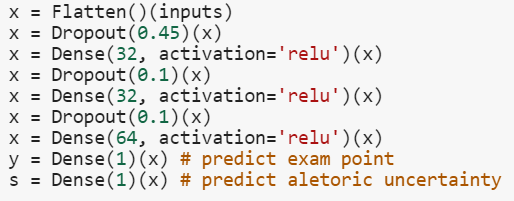
\includegraphics[width=0.7\textwidth]{images/methodpictures/uncert-net-ffm234.PNG}
    \caption{Nätverksstrukturen för osäkerhetsnätverket i FFM234. (PLACEHOLDER)}
    \label{fig:uncert_net_ffm234}
\end{figure}

\begin{figure}[h]
    \centering
    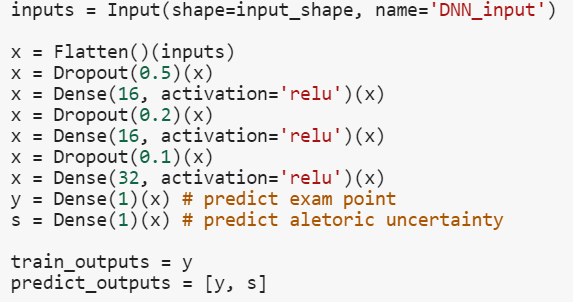
\includegraphics[width=0.7\textwidth]{images/methodpictures/uncert-net-ffm521.PNG}
    \caption{Nätverksstrukturen för osäkerhetsnätverket i FFM521. (PLACEHOLDER)}
    \label{fig:uncert_net_ffm521}
\end{figure}

\section{Utformning av experiment för interaktion mellan student och artificiell intelligens}